%&../settings/preamble.main

\ifsubfile
\usepackage{../settings/subfile}
\setcounter{chapter}{14}

% arara: pdflatex: { options: ["--output-directory=../build"], draft: yes, synctex: no }
% arara: pdflatex: { options: ["--output-directory=../build"], synctex: no }
\begin{document}
\fi
\chapter{Algoritmi ingordi}
\epigraph{`The point is, ladies and gentleman, that greed, for lack of a better word, is good. %
           Greed is right, greed works. %
           Greed clarifies, cuts through, and captures the essence of the evolutionary spirit. %
           Greed, in all of its forms; greed for life, for money, for love, for knowledge has marked the upward surge of mankind.''}%
         {--- \textup{\textsc{Gordon Gekko, Wall Street (1987)}}}

\begin{note}
Non è difficile scrivere algoritmi ingordi, la parte difficile sta nel dimostrare che restituiscano la soluzione ottimale.
\end{note}

Molti dei problemi che vedremo li abbiamo già visti, ma in questo capitolo tratteremo dei loro casi particolari.
Capita spesso che per risolvere casi generali ci si debba avvalere della programmazione dinamica, mentre per casi particolari sia meglio usare algoritmi ingordi.

\section{Introduzione}

Sia la programmazione dinamica che gli algoritmi greedy cercano di risolvere problemi di ottimizzazione.
Gli algoritmi che li risolvono devono prendere una serie di decisioni e differiscono fra di loro da \emph{come} queste decisioni vengono prese.
Nella programmazione dinamica valutiamo tutte le possibili decisioni evitando di rivalutare decisioni (percorsi) già intraprese.
Negli algoritmi ingordi, invece, selezioniamo \emph{una sola} fra le possibili decisioni. Quale? Quella che sembra ottima (ovvero \emph{localmente ottima}).
\`{E} però necessario dimostrare che si ottiene un ottimo globale (ossia una soluzione \emph{globalmente ottima}).

\begin{note}
Questo approccio riduce la complessità di dover valutare tutte le possibilità, ma necessita di essere dimostrato.
\end{note}

\paragraph{Quando applicarla}
\`{E} consigliato applicare la tecnica greedy quando fra tutte le scelte possibili ne può essere individuata una che porta sicuramente alla soluzione ottima.
Deve comunque rimanere valida (come nella programmazione dinamica) la proprietà di \emph{sottostruttura ottima} ovvero che quando viene effettuata una scelta resti un sottoproblema con la stessa struttura del problema principale.

\begin{note}
Non tutti i problemi hanno una soluzione greedy.
\end{note}

\section{Insieme indipendente di intervalli non pesati}

\paragraph{Definizione del problema}
Dati in input un insieme di intervalli della retta reale \(S = \{1, 2, \dots n\}\).
Trovare un \emph{insieme indipendente massimale}, ovvero un sottoinsieme di cardinalità massima formato da intervalli disgiunti tra loro.

\begin{note}[Proprietà degli intervalli]
Gli intervalli sono chiusi a sinistra e aperti a destra.
\end{note}

% TODO link a insieme indipendente di intervalli pesati
Abbiamo già risolto questo problema (con la programmazione dinamica), ma il fatto che tutti i pesi siano pari a 1 porta ad una semplificazione del problema.

\begin{figure}[bt]
	\centering
	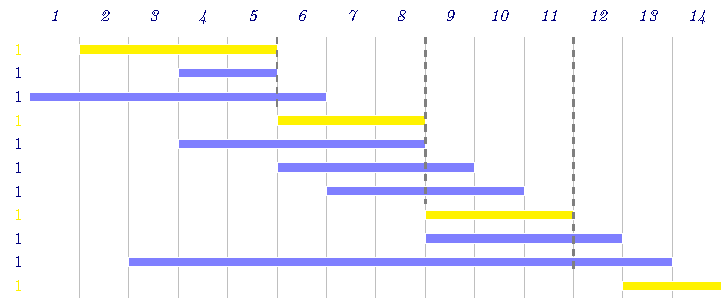
\includegraphics{gantt-greedy}
	\caption[]{Una delle possibili soluzioni ingorde al problema dell'insieme indipendente di intervalli.
			   Quali altre possibili soluzioni di cardinalità massima sono presenti?
			   Nota che tutti gli intervalli hanno lo stesso peso.}%
	\label{fig:gantt-solution-greedy}
\end{figure}

\begin{note}
Per questo particolare problema non esiste un insieme di cardinalità 5 (ossia un insieme contenente cinque elementi).
\end{note}

\paragraph{Come affrontare il problema}
\begin{enumerate}
	\item \emph{individuare} la sottostruttura ottima;
	\item \emph{scrivere} una definizione ricorsiva per la dimensione della soluzione ottima;
	\item \emph{cercare} una possibile scelta ingorda;
	\item \emph{dimostrare} che la scelta presa porti alla soluzione ottima;
	\item \emph{scrivere} un algoritmo ricorsivo (spesso sono iterativi) che effettui sempre la scelta ingorda.
\end{enumerate}

\subsection{Individuazione sottostruttura ottima}

Assumiamo che gli intervalli siano ordinati per tempo di fine (\(b_1 \leqslant b_2 \leqslant \dots b_n\)).

Definiamo il sottoproblema \(S[i,j]\) come l'insieme di intervalli che iniziano dopo la fine di \(i\) e finiscono prima dell'inizio di \(j\), ovvero \(S[i,j] = \{ k \mid b_i \leqslant a_k < b_k \leqslant a_j \}\).

Per scopi implementativi (fungeranno da sentinelle) aggiungiamo due intervalli fittizi che singoleggiano \(\pm\infty\), ovvero l'intervallo zeresimo indicato da \(b_0\) (\(b_0 = -\infty\)) e l'intervallo successivo indicato da \(n+1\) (\(n+1 = +\infty\)).
In questi termini il problema iniziale corrisponde al problema \(S[0, n+1]\).

\begin{note}
L'idea è definire problemi a mano a mano sempre più piccoli.
E definirli in base agli indici degli intervalli rimanenti.
\end{note}

\begin{theorem}
Supponiamo che \(A[i,j]\) sia una (poiché non è unica) soluzione ottimale di \(S[i,j]\) e sia \(k\) un (qualunque) intervallo che appartiene a \(A[i,j]\); suddividiamo quindi il problema \(S[i,j]\) in due sottoproblemi:

\begin{itemize}
	\item \(S[i,k]\): gli intervalli di \(S[i,j]\) che finiscono prima di \(k\);
	\item \(S[k,j]\): gli intervalli di \(S[i,j]\) che iniziano dopo di \(k\)
\end{itemize}

\(A[i,j]\) contiene le soluzioni ottimali di \(S[i,k]\) e \(S[k,j]\) quindi:

\begin{itemize}
	\item \(A[i,j] \cap S[i,k]\) è la soluzione ottimale di \(S[i,k]\)
	\item \(A[i,j] \cap S[k,j]\) è la soluzione ottimale di \(S[k,j]\)
\end{itemize}
\end{theorem}

\begin{proof}[Dimostrazione per assurdo]
Se esistesse una soluzione migliore al problema \(S[i,j]\), diciamo \(A'[i,k]\) e la sostituissi ad \(A[i,k]\) ottenerrei una soluzione migliore anche al mio problema originale, ma questo non è possibile poiché se ottenessi una soluzione migliore allora \(A[i,k]\) non sarebbe una soluzione ottima, il che è assurdo.
\end{proof}

\subsection{Definizione ricorsiva del costo della soluzione}

Partendo dalla definizione ricorsiva della soluzione

\begin{equation*}
A[i,j] = A[i,k] \cup \{ k \} \cup A[k, j]
\end{equation*}

\noindent
non possiamo determinare \(k\) a priori quindi dobbiamo necessariamente provare tutti i valori.

L'equazione di ricorrenza che si ottiene è la seguente

\begin{equation*}
	DP[i,j] =
	\begin{dcases}
		0 & S[i,j] = \emptyset \\
		\max_{k \in S[i,j]} \{ \underbracket[1pt]{DP[i,k]}_{\text{prima di }k} + \underbracket[1pt]{DP[k,j]}_{\text{dopo }k} + 1 \} & \textrm{altrimenti} \\
	\end{dcases}
\end{equation*}
dove \(DP[i, j]\) è la dimensione del più grande sottoinsieme \(A[i,j] \subseteq S[i,j]\) di intervalli indipendenti.

\begin{enumerate}
	\item se l'insieme di intervalli dati in input è vuoto (\(S[i,j] = \emptyset\)), allora la dimensione dell'insieme è pari a \(0\) (caso base);
	\item altrimenti, se l'insieme di intervalli di partenza non è vuoto, consideriamo l'insieme di cardinalità massima.
	L'insieme viene calcolato scegliendo l'intervallo \(k\)-esimo fra tutti gli intervalli \(k\) appartenenti all'insieme di partenza (\(k \in S[i,j]\)), sommando quindi \(1\) alla soluzione finale, e chiamando ricorsivamente il problema sugli intervalli rimanenti.
\end{enumerate}

\subsection{Verso una soluzione ingorda}

La definizione precedente ci permette di scrivere un algoritmo basato su programmazione dinamica o su memoization di complessità \(\Omicron(n^3)\): bisogna necessariamente risolvere tutti i problemi con \(i<j\), con costo \(\Omicron(n)\) nel caso pessimo.

Nella risoluzione del problema di intervalli \emph{pesati} abbiamo visto un algoritmo di complessità \(\Omicron(n \log n)\), il quale è applicabile anche nella risoluzione di questo problema.
Questa complessità era data dall'ordinamento del vettore che avveniva prima che i dati venissero processati indipendentemente dall'ordinamento iniziale.
Tuttavia è possibile migliorare il nostro algoritmo cercando una soluzione ingorda al nostro problema evitando di valutare tutte le possibili soluzioni.
Infatti non è necessario analizzare tutti i possibili valori di \(k\).

\begin{theorem}[scelta ingorda]

Sia \(S[i,j]\) un sottoproblema non vuoto, ed indentifichiamo \(m\) l'intervallo di \(S[i,j]\) con il \textcolor{darker}{minor tempo di fine}, allora:

\begin{enumerate}
	\item il sottoproblema \(S[i,m]\) è vuoto;
	\item \(m\) è compreso in \underline{qualche} soluzione ottima di \(S[i,j]\).
\end{enumerate}

\end{theorem}

\subsection{Dimostrazione che è una soluzione ottima}

\begin{proof}
Fai riferimento \href{https://youtu.be/pt53LdiwN7s?t=1381}{alla spiegazione su youtube} qui non riportata (importante).
\end{proof}

\paragraph{Conseguenze}
Non è più necessario analizzare tutti i possibili valori di \(k\) in quanto faccio una una scelta \enquote{ingorda}, ma sicura: seleziono l'attività \(m\) con il minor tempo di fine.
A questo punto non è più necessario analizzare due sottoproblemi; eliminando tutte le attività che non sono compatibili con la scelta ingorda mi resta solo il sottoproblema \(S[m,j]\) da risolvere.

\subsection{Scrittura dell'algoritmo}

\begin{algorithm}[H]
	\caption{Insieme indipendente di intervalli disgiunti}
	%&../preamble

% arara: pdflatex: { synctex: no }
% arara: latexmk: { clean: partial }
\ifstandalone
\begin{document}
\begin{algorithm}[H]
\fi

\prototype{\Set \independentSet{\Array{\Int} \(a\), \Array{\Int} \(b\)}}{

	\BlankLine
	\{ ordina \(a\) e \(b\) in modo che \(b[1] \leqslant b[2] \leqslant \cdots \le b[n]\) \}\;
	\tcp{\(\Omicron(n)\) se già ordinati, \(\Omicron(n \log n)\) altrimenti}

	\BlankLine
	\Set \(S \Assign \setConstructor\)\;
	\(S\).\setInsert(1) \Comment*[h]{inserisco il primo intervallo}\;
	\Int \Last \(\Assign 1\) \Comment*[h]{ultimo intervallo inserito}\;

	\BlankLine
	\From{\(i \Assign 2\) \DownTo \(n\)}{
		\If{\(a[i] \geqslant b[\Last]\)}{
			\tcp{gli intervalli sono indipendenti}

			\BlankLine
			\(S\).\setInsert(i) \Comment*[h]{lo inserisco}\;
			\(\Last \Assign i\) \Comment*[h]{lo rendo l'ultimo inserito}\;
		}
	}

	\Return \(S\)\;
}

\ifstandalone
\end{algorithm}
\end{document}
\fi

\end{algorithm}

\paragraph{Commento}
Divido il resto per il taglio della moneta più grande trovando il numero di monete massimo di quel taglio, dopodiché tolgo il valore della somma quelle monete dal resto.

\begin{note}
Questo algoritmo non è applicabile al problema dell'insieme indipendente di intervalli \emph{pesati}.
\end{note}

\paragraph{Ricapitolando}
Abbiamo cercato di risolvere il problema della selezione delle attività tramite programmazione dinamica, prima individuando una sottostruttura ottima, poi scrivendo una definizione ricorsiva per la dimensione della soluzione ottima.

Abbiamo poi dimostrato la proprietà della scelta greedy: dimostrando che per ogni sottoproblema, esiste almeno una soluzione ottima che contiene la scelta greedy.
Infine abbiamo scritto un algoritmo iterativo che effettua sempre la scelta ingorda.

\section{Resto}

\paragraph{Definizione del problema}
Dati in input un insieme di \enquote{tagli} di monete, memorizzati in un vettore di interi positivi \(t[1 \ldots n]\) ed un intero \(R\) rappresentante il resto che dobbiamo restituire.
Trovare il più piccolo numero intero di pezzi necessari per dare un resto di \(R\) centesimi utilizzando i tagli di cui sopra, assumendo di avere un numero illimitato di monete per ogni taglio.

Più formalmente bisogna trovare un vettore \(x\) di interi non negativi tale che
\begin{align*}
R &= \sum_{i=1}^n x[i] \cdot t[i] & m &= \sum_{i=1}^n x[i] \quad \textrm{è minimo} \\
\end{align*}

\subsection{Individuazione sottostruttura ottima}

Sia \(S(i)\) il problema di dare il resto pari ad \(i\).
Sia \(A(i)\) una soluzione ottima del problema \(S(i)\), rappresentata da un multi-insieme (un insieme nel quale lo stesso indice può comparire più di una volta); sia \(j \in A(i)\) (\(j\) un possibile taglio).
Allora, \(S(i-t[j])\) è un sottoproblema di \(S(i)\), la cui soluzione ottima è data da \(A(i) - \{j\}\).

Quest'idea si traduce nella seguente definizione ricorsiva.

\subsection{Definizione ricorsiva del costo della soluzione}

Utilizziamo la tabella \(DP[0 \ldots R]\) per memorizzare le soluzioni e in \(DP[i]\) memorizziamo il minimo numero di monete per risolvere il problema \(S[i]\).

\begin{equation*}
	DP[i] =
	\begin{dcases}
		0 & i = 0 \\
		\min_{1 \leqslant j \leqslant n} \{ DP[i-t[j]] \text{ t.c.\ } t[j] \leqslant i \} + 1 & i > 0
	\end{dcases}
\end{equation*}

Il numero minimo di monete è \(0\) se non dobbiamo dare nessun resto (caso base), altrimenti cerchiamo fra tutti i possibili tagli quello che minimizza il numero di monete restituite.

\subsection{Algoritmo basato su programmazione dinamica}

\begin{algorithm}[H]
	\caption{Programmazione dinamica applicata al problema del resto}
	%&../preamble

% arara: pdflatex: { synctex: no }
% arara: latexmk: { clean: partial }
\ifstandalone
\begin{document}
\begin{algorithm}[H]
\fi

\prototype{\restoDP{\Array{\Int} t, \Int n, \Int R}}{
	\params{t}[tagli disponibili]
	\params{n}[numero di monete]
	\params{R}[il resto da dare]

	\BlankLine
	\BlankLine
	\(DP\) \Assign \new \Array{\Int}[0][R]\;
	\(S\) \Assign \new \Array{\Int}[0][R]\;
	\(DP[0] \Assign 0\) \Comment*[h]{caso base}\;

	\BlankLine
	\tcp{Riempire la tabella \(DP\)}
	\From{\(i \Assign 1\) \DownTo \(R\)} {
		\(DP[i] \Assign +\infty\)\;

		\BlankLine
		\BlankLine
		\From(\Comment*[h]{Riempio la tabella}){\(j \Assign 1\) \DownTo \(n\)} {
			\If{\(t[j] \leqslant i\) \And \(DP[i-t[j]] + 1 < DP[i]\)}{
				\tcp{aggiorno il valore}

				\BlankLine
				\(DP[i] \Assign DP[i - t[j]] + 1\) \Comment*[h]{registro il valore}\;
				\(S[i] \Assign j\) \Comment*[h]{la moneta da utilizzare per risolvere il problema quando il taglio è \(i\)}\;
			}
		}
	}

	\BlankLine
	\While(\Comment*[h]{ho resto da dare}){\(R > 0\)}{
		\Print \(t[S[R]]\) \Comment*[h]{stampo la moneta}\;
		\(R \Assign R - t[S[R]]\) \Comment*[h]{decremento il resto}\;
	}
}

\ifstandalone
\end{algorithm}
\end{document}
\fi

\end{algorithm}

\paragraph{Commento}
\(t[j] \leqslant i\) sta a significare che il taglio delle monete che possiamo scegliere dev'essere più piccolo del resto che dobbiamo dare.

\paragraph{Complessità}
\(\Omicron(nR)\) dato dai cicli innestati.
Una soluzione dipendente dal resto \(R\) da dare non è ottimale, si può fare meglio di così.

\begin{note}
Quest'algoritmo rappresenta la soluzione generale al problema e, a differenza dell'algoritmo ingordo (che vedremo più avanti), funziona per qualsiasi insieme di tagli di monete.
\end{note}

\subsection{Scelta ingorda}

Seleziona la moneta \(j\) \textcolor{darker}{più grande} tale per cui \(t[j] \leqslant R\), per poi risolvere il problema \(S(R - t[j])\).

\subsection{Scrittura dell'algoritmo}

\begin{algorithm}[H]
	\caption{Approccio ingordo al problema del resto}
	%&../preamble

% arara: pdflatex: { synctex: no }
% arara: latexmk: { clean: partial }
\ifstandalone
\begin{document}
\begin{algorithm}[H]
\fi

\prototype{\restoGreedy{\Array{\Int} \(t\), \Int \(n\), \Int \(R\), \Array{\Int} \(x\)}}{

	\{ Ordina le monete in modo \emph{decrescente} \}\;
	\tcp{\(\Omicron(n)\) se già ordinato, \(\Omicron(n \log n)\) altrimenti}

	\BlankLine
	\From(\Comment*[h]{\(\Omicron(n)\)}){\(i \Assign 1\) \DownTo \(n\)} {

		\BlankLine
		\tcp{il numero di monete di taglio massimo}
		\(x[i] \Assign \left\lfloor \dfrac{R}{t[i]} \right\rfloor\)\;

		\BlankLine
		\tcp{calcolo il resto rimanente}
		\(R \Assign R - x[i] \cdot t[i]\)\;
	}

	\Return \(R\)
}

\ifstandalone
\end{algorithm}
\end{document}
\fi

\end{algorithm}

\paragraph{Complessità}
Questo algoritmo ha complessità lineare, ossia \(\Omicron(n)\).

\subsection{Dimostrazione che è una soluzione ottima}

\begin{note}
La seguente dimostrazione si riferiscere ai tagli \({\myCircle}_1 = 50\), \({\myCircle}_2 = 10\), \({\myCircle}_3 = 5\), \({\myCircle}_4 = 1\).
\end{note}

Sia \(x\) una qualunque soluzione ottima; quindi il resto \(R\) è esprimibile tramite una certa somma dei nostri possibili tagli, dove il numero dei tagli \(m\) è minimo:
\begin{align*}
R &= \sum_{i=1}^n x[i] \cdot t[i] & m &= \sum_{i=1}^n x[i] \\
\end{align*}

\noindent
Sia \(m_k\) \emph{la somma delle monete di taglio inferiore} a \(t[k]\):
\begin{equation*}
m_k = \sum_{i=k+1}^{4} x[i] \cdot t[i]
\end{equation*}

\noindent
Se dimostriamo che la somma delle monete di taglio inferiore a \(k\) è minore del valore del taglio \(k\)-esimo (\(\forall k: m_k < t[k]\)), allora la soluzione (ottima) è proprio quella calcolata dall'algoritmo.

\(m_{*}\) denota l'insieme di monete con tagli inferiore a \({\myCircle}_{*}\) centesimi, ad esempio \(m_{2}\) denota l'insieme di monete con tagli inferiore a (\({\myCircle}_{2} =\)) 10 centesimi.
Mentre \(x[*]\) simboleggia il \emph{numero} di monete di quel taglio presenti nel resto della soluzione ottima, ad esempio \(x[3]\) simboleggia il \emph{numero} di monete di \({\myCircle}_3 = 5\) centesimi.
\begin{align*}
m_4 &= 0					&&< 1 = t[4] \\
m_3 &= 1 \cdot x[4]			&& < 5 = t[3] \\
m_2 &= 5 \cdot x[3] + m_3	&&\leqslant 5 + m_3 < 5 + 5 = 10 = t[2] \\
m_1 &= 10 \cdot x[2] + m_2	&& \leqslant 40 + m_2 < 40 + 10 = 50 = t[1] \\
\end{align*}

\begin{note}
Fare riferimento \href{https://youtu.be/pt53LdiwN7s?t=2779}{alla spiegazione su youtube} qui non riportata.
\end{note}

\section{Approccio ingordo}

Cercheremo di risolvere i successivi problemi avendo direttamente un approccio ingordo, senza passare prima per la programmazione dinamica.
Come fare? bisogna:
\begin{itemize}
	\item \emph{evidenziare} i passi di decisione, \emph{trasformando} il problema di ottimizzazione in un problema di \enquote{scelte} successive;
	\item \emph{evidenziare} una possibile scelta ingorda, \emph{dimostrando} che tale scelta rispetta il principio di scelta ingorda;
	\item \emph{evidenziare} la sottostruttura ottima, \emph{dimostrando} che la soluzione ottima del problema \enquote{residuo} dopo la scelta ingorda può essere unito a tale scelta;
	\item \emph{scrivendo} un algoritmo top-down (anche iterativo), in alcuni casi sarà necessario pre-processare l'input.
\end{itemize}

\section{Scheduling}

\paragraph{Definizione del problema}
Supponiamo di avere un processore e \(n\) job da eseguire su di esso,
ognuno caratterizzato da un tempo di esecuzione \(t[i]\) noto a priori.
Trovare una sequenza di esecuzione (permutazione) che minimizzi il \emph{tempo di completamento medio}.

Dato un vettore \(A[1 \ldots n]\) contenente una permutazione di \(\{ 1, \ldots n \}\), il \emph{tempo di completamento} dell'\(h\)-esimo job nella permutazione è:
\begin{equation*}
T_A(h) = \sum_{i=1}^h t[A[i]]
\end{equation*}

Ad esempio
% NOTE: tex.stackexchange.com/questions/296387/
% TODO: isolare
% \documentclass[tikz,border=2pt]{standalone}
\begin{figure}[H]
	\centering
	\begin{tikzpicture}[thick, font = \ttfamily\bfseries]
		\node[job, minimum width = 2.0cm] at (0,0)   { 4 };
		\node[job, minimum width = 0.5cm] at (2,0)   { 1 };
		\node[job, minimum width = 3.0cm] at (2.5,0) { 6 };
		\node[job, minimum width = 1.5cm] at (5.5,0) { 3 };
		\node[] at (0,	-0.50){0};
		\node[] at (2,	-0.50){4};
		\node[] at (2.5,-0.50){5};
		\node[] at (5.5,-0.50){11};
		\node[] at (7,	-0.50){14};
	\end{tikzpicture}
\end{figure}
\noindent
dove il tempo di completamento medio è pari a \[\frac{4+5+11+14}{4} = \frac{34}{4} = 8.5\]

Applicando l'algoritmo \emph{Shortest Job First}:

\begin{figure}[H]
	\centering
	\begin{tikzpicture}[thick, font = \ttfamily\bfseries]
		\node[job, minimum width = 0.5cm] at (0.0,0) { 1 };
		\node[job, minimum width = 1.5cm] at (0.5,0) { 3 };
		\node[job, minimum width = 2.0cm] at (2.0,0) { 4 };
		\node[job, minimum width = 3.0cm] at (4.0,0) { 6 };
		\node[] at (0.0, -0.50){0};
		\node[] at (0.5, -0.50){1};
		\node[] at (2.0, -0.50){4};
		\node[] at (4.0, -0.50){8};
		\node[] at (7,   -0.50){14};
\end{tikzpicture}
\end{figure}

dove il tempo di complemento è pari a \[\frac{1+4+8+14}{4} = \frac{27}{4} = 6.75 < 8.5\]

\begin{theorem}[Scelta greedy]
Esiste una soluzione ottima \(A\) in cui il job con minor tempo di fine \(m\) si trova in prima posizione (\(A[1] = m)\).
\end{theorem}

\begin{theorem}[Sottostruttura ottima]
Sia \(A\) una soluzione ottima di un problema con \(n\) job, in cui il job con minor tempo di fine \(m\) si trova in prima posizione.
La permutazione dei seguenti \(n-1\) job in \(A\) è una soluzione ottima al sottoproblema in cui il job \(m\) non viene considerato.
\end{theorem}

\subsection{Dimostrazione}

Fai riferimento \href{https://youtu.be/pt53LdiwN7s?t=3626}{alla spiegazione grafica su youtube} qui non riportata.

\section{Zaino frazionario}

Riproponiamo un problema visto in precedenza, ma stavolta anzichè avere la limitazione di poter prenderere o non prendere un oggetto (chiamato problema dello zaino \texttt{0/1}), possiamo prenderne anche frazioni di esso (zaino \emph{reale}).

Un approccio ingordo è quello di ordinare gli oggetti in ordine di \emph{profitto specifico decrescente} (profitto su volume) e prendere quante più frazioni possibili degli elementi fino a riempire l'intera capacità dello zaino.

\begin{algorithm}[H]
	\caption{Approccio ingordo al problema del resto}
	%&../preamble

% arara: pdflatex: { synctex: no }
% arara: latexmk: { clean: partial }
\ifstandalone
\begin{document}
\begin{algorithm}[H]
\fi

\prototype{\zaino{\Array{\Real} \(p\), \Array{\Real} \(v\), \Real \(C\), \Int \(n\), \Array{\Real} \(x\)}}{

	\BlankLine
	\{ ordina \(p\) e \(v\) in modo che \(\frac{p[1]}{w[1]} \geqslant \frac{p[2]}{w[2]} \geqslant \cdots \geqslant \frac{p[n]}{w[n]}\)\}\;

	\BlankLine
	\tcp{\(\Omicron(n)\) se già ordinato, \(\Omicron(n \log n)\) altrimenti}

	\BlankLine
	\BlankLine
	\From{\(i \Assign 1\) \DownTo \(n\)}{
		\(x[i] \Assign \MathMin\left( \dfrac{C}{w[i]}, 1 \right)\) \Comment*[h]{ne prendo solo una frazione?}\;

		\BlankLine
		\(C \Assign C - x[i] \cdot w[i]\) \Comment*[h]{aggiorno la capacità residua}\;
	}
}

\ifstandalone
\end{algorithm}
\end{document}
\fi

\end{algorithm}

\(x[i]\) rappresenta la frazione dell'oggetto \(i\)-esimo che deve essere presa.

\subsection{Correttezza dell'algoritmo}

Dimostrazione informale:
\begin{enumerate}
	\item assumiamo che gli oggetti siano ordinati per profitto specifico decrescente;
	\item sia \(x\) una soluzione ottima;
	\item supponiamo che \(x[1] < \min\left( \frac{C}{w[i]}, 1 \right) < 1\);
	\item allora possiamo costruire una nuova soluzione in cui \(x'[1] = \min\left( \frac{C}{w[i]}, 1 \right)\) e la proporzione di uno o più oggetti è ridotta di conseguenza;
	\item otteniamo così una soluzione \(x'\) di profitto uguale o superiore, visto che il profitto specifico del primo oggetto è massimo.
\end{enumerate}

\section{Compressione di Huffman}

Per rappresentare in modo efficiente i dati (minimizzare lo spazio su disco occupato, minimizzare il tempo di trasferimento su disco\dots ) abbiamo bisogno di adottare una qualche tecnica di compressione.
Una fra le tante possibili è la \emph{codifica dei caratteri}.

\begin{note}
La codifica dei caratteri ha una complessità dipendente in percentuale dalle dimensioni del file di origine.
\end{note}

\begin{note}
Un codice non deve essere mai \underline{prefisso} di un altro codice, in quanto è una condizione necessaria per distinguerli.
\end{note}

\subsection{Rappresentazione ad albero per la decodifica}

Rappresenteremo il nostro risultato tramite un albero.
La rappresentazione sulla sinistra non è la migliore possibile.
Ed è possibile ottimizzare l'albero comprimendo i cammini per i caratteri \texttt{d} e \texttt{e} (come puoi vedere nella figura a destra).
Modificando di conseguenza anche la codifica dei caratteri ed ottenendo una codifica ottimizzata.

\begin{minipage}[t]{.5\linewidth}
\begin{figure}[H]
	\centering
	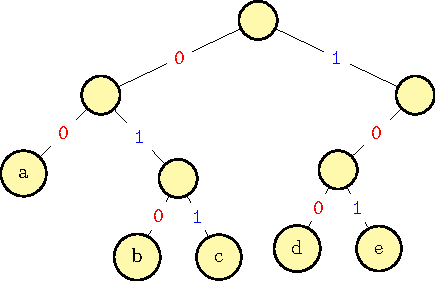
\includegraphics{treenode}
\end{figure}
\centering
{\ttfamily
\begin{tabular}{|c|c|c|c|c|}\hline
	a & b & c & d & e  \\\hline
	\R{0}\R{0} & \R{0}\B{1}\R{0} & \R{0}\B{1}\B{1} & \B{1}\R{0}\R{0} & \B{1}\B{1}\B{1} \\\hline
\end{tabular}}
\end{minipage}
\begin{minipage}[t]{.5\linewidth}
\begin{figure}[H]
	\centering
	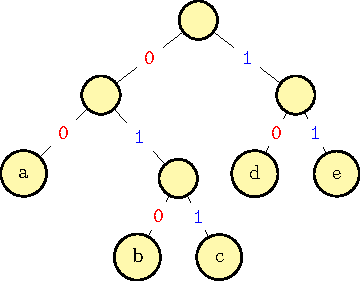
\includegraphics{treenode-compressed}
\end{figure}
\centering
{\ttfamily
\begin{tabular}{|c|c|c|c|c|}\hline
	a & b & c & d & e  \\\hline
	\R{0}\R{0} & \R{0}\B{1}\R{0} & \R{0}\B{1}\B{1} & \B{1}\R{0} & \B{1}\B{1} \\\hline
\end{tabular}}
\end{minipage}

\vspace{10pt}
\paragraph{Definizione formale del problema}
Dati in input un file \(F\) composto da caratteri di un certo alfabeto (che chiameremo \(\Sigma\)).
Dobbiamo cercare di rappresentare il nostro file con il minor numero di bit possibili.
Supponiamo che l'albero \(T\) rappresenti la nostra codifica.
Per ogni carattere appartente all'alfabeto (\(c \in \Sigma\)), definiamo come \(d_{T}(c)\) la profondità della foglia che rappresenta il carattere \(c\).
Quindi il codice per rappresentare \(c\) richiederà \(d_{T}(c)\) bit.
Infine se \(f[c]\) è il numero di occorrenze di \(c\) in \(F\), allora la \emph{dimensione della codifica} è
\begin{equation*}
C[F,T] = \sum_{c \in \Sigma} f[c] \cdot d_{T}(c)
\end{equation*}

\begin{itemize}
	\item \(f[c]\): frequenza del carattere \(c\) nell'alfabeto \(\Sigma\);
	\item \(d_{T}(c)\): profondità del nodo \(c\) nell'albero \(T\), ovvero i bit necessari per la codifica di \(c\).
\end{itemize}
Quindi una codifica \(C\) è data da un particolare albero \(T\) dove viene rappresentata e da un particolare file \(F\).

\subsection{Principio dell'algoritmo di Huffman}

Vogliamo minimizzare la lunghezza della codifica per caratteri che compaiono più frequentemente: assegnando ai caratteri con frequenza minore codici corrispondenti a percorsi più lunghi all'interno dell'albero e a quelli di frequenza maggiore un percorso più corto.

\begin{note}
Una certa codifica è progettata per un file specifico.
\end{note}

\subsection{Algoritmo}

\begin{algorithm}[H]
	\caption{Approccio ingordo al problema del resto}
	%&../preamble

% \documentclass[varwidth=6in]{standalone}
% \usepackage{../preamble}

% arara: pdflatex: { synctex: no }
% arara: latexmk: { clean: partial }
\ifstandalone
\begin{document}
\NoCaptionOfAlgo
\begin{algorithm}[H]
\caption[Algoritmo di Huffman]{}
\fi

\prototype{\Tree \huffman{\Array{\Int} \(c\), \Array{\Int} \(f\), \Int \(n\)}}{
	\tcp{\Array{c}{1}{n}: caratteri dell'alfabeto}
	\tcp{\(f[1 \dots n]\): frequenze dei caratteri}
	\tcp{\(n\): dimensione dell'alfabeto}

	\BlankLine
	\Heap \(Q\) \Assign \minHeapConstructor\;

	\BlankLine
	\From(\Comment*[h]{}{\(\Omicron(n)\)}){\(i \Assign 1\) \DownTo \(n\)}{
		\(Q\).\heapInsert{\(f[i]\), \treeConstructor{\(f[i]\), \(c[i]\)}} \Comment*[h]{}{\(\Omicron(\log n)\)}
	}

	\BlankLine
	\From(\Comment*[h]{\(n\): radice}{\(\Omicron(n)\)}){\(i \Assign 1\) \DownTo \(n-1\)}{
		\BlankLine
		\tcp{estraggo i 2 caratteri meno frequenti}
		\(z_1\) \Assign \(Q\).\heapDeleteMin\;
		\(z_2\) \Assign \(Q\).\heapDeleteMin\;

		\BlankLine
		\tcp{Creo un nuovo nodo}
		\(z \Assign \treeConstructor(z_1.f + z_2.f, \Nil)\)\;
		\(z.\varLeft \Assign z_1\)\;
		\(z.\varRight \Assign z_2\)\;

		\BlankLine
		\tcp{Lo inserisco nella coda}
		% \marginnote{\color{blue} \(\Omicron(\log n)\)}
		\(Q\).\heapInsert{z.f, z}\;
	}

	\Return \(Q\).\heapDeleteMin\;
}

\ifstandalone
\end{algorithm}
\RestoreCaptionOfAlgo
\end{document}
\fi

\end{algorithm}

Siccome ogni volta devo estrarre i due elementi più piccoli faccio affidamento ad una {\minHeapConstructor}.

1. inserisco tutte le lettere con la priorità data dalla loro frequenza e con un nodo contenente sia la frequenza che la lettera associata.
Dopodiché estraggo i due elementi più piccoli, credo un nuovo nodo contenente i due elementi appena estratti e restituisco il nodo così fatto al chiamante.

\paragraph{Funzionamento dell'algoritmo}
\begin{enumerate}
	\item rimuovo i due nodi con frequenza minore;
	\item creo un nodo un'etichetta nulla e con frequenza pari alla somma delle frequenze dei nodi eliminati;
	\item collego i due nodi con il nodo creato;
	\item aggiungo il nodo così creato alla lista, mantenendo l'ordine;
	\item si termina quando reasta un solo nodo nella lista;
	\item al termine, si etichettano gli archi dell'albero con bit \texttt{0}, \texttt{1}.
\end{enumerate}

\paragraph{Complessità}
Effettuo \(n\) volte operazioni che costano \(\log n\), come le operazioni di {\heapInsert} o di {\heapDeleteMin} per una complessità totale di \(\Omicron(n \log n)\).

\subsection{Dimostrazione di correttezza}

\begin{theorem}
L'output dell'algoritmo Huffman per un dato file è un codice a prefisso ottimo.
\end{theorem}

Scegliere i due elementi con la frequenza più bassa conduce sempre ad una soluzione ottimale.
Dato un problema sull'alfabeto \(\Sigma\).
\`{E} possibile costruire un sottoproblema con un alfabeto più piccolo in cui togliamo due caratteri e ne aggiungiamo uno fittizio.

\subsection{Scelta ingorda}

\texttt{MATERIALE MANCANTE}

\section{Albero di copertura minimi}

\paragraph{Problema}
Dato un grafo pesato, determinare come interconnettere tutti i suoi nodi minimizzando il costo del peso associato ai suoi archi (agli archi che andiamo a scegliere).
Questo problema prende vari nomi, come albero di copertura minimo o albero di connessione minimo, in inglese \emph{Minimum Spanning Tree}.

\paragraph*{Risorse}

\begin{otherlanguage}{english}
If you are curious about who is the cookie monster, then watch the \href{https://www.youtube.com/watch?v=tKwnms5iRBU}{MIT lecture on Minimum Spanning Tree} of Professor Erik Demaine.
\end{otherlanguage}
% Questo materiale è basato sulla lezione \enquote{\href{https://www.youtube.com/watch?v=VocW2D-Z0hk}{Alberi di copertura di peso minimo}} di \href{http://cricca.disi.unitn.it/montresor/}{Alberto Montresor}.

% \colon -> tex.stackexchange.com/questions/37789
\paragraph{Definizione del problema}
Dati in input un grafo non orientato e connesso \(G = (V, E)\) ed una funzione di peso (che determina il costo di connessione) \(w\colon V \times V \to\! \mathbb{R}\) (data una coppia di nodi restituisce un numero reale che rappresenta il peso).

\begin{note}
Poiché \(G\) non è orientato possiamo dire che \(w(u,v) = w(v,u)\).
\end{note}

Un albero di copertura di \(G\) è un sottografo \(T = (V, E_{T})\) tale che \(T\) è un albero non radicato, i lati dell'albero siano un sottoinsieme di quelli del grafo (\(E_{T} \subseteq E\)) e che contenga tutti i vertici di \(G\).
Il problema consiste quindi nel trovare l'albero di copertura il cui \emph{peso totale} sia minimo rispetto a ogni altro albero di copertura, dove il \emph{peso totale} è dato da:
\begin{equation*}
w(T) = \sum_{\mathclap{e \in T}}\; w(e) = \sum_{\mathclap{[u,v] \in E_T}}\; w(u,v)
\end{equation*}

\begin{note}
Non è detto che l'albero di copertura minimo sia univoco.
\end{note}

\subsection{Algoritmo generico}

L'idea è di accrescere un sottoinsieme \(A\) di archi in modo tale che venga sempre
rispettata la seguente invariante: \(A\) è un sottoinsieme di qualche albero di connessione minimo.

\begin{theorem}[Arco sicuro]
Un arco \([u,v]\) è detto sicuro per \(A\) se \(A \cup \{[u,v]\}\) è ancora un sottoinsieme di qualche albero di connessione minimo.
\end{theorem}

\begin{algorithm}[H]
\caption{Algoritmo generico per generare un albero di copertura minimo}

\prototype{\Set \mstGenerico{\Graph G, \Array{\Int} w}}{

	\Set \(A \Assign \emptyset\) \Comment*[h]{parto da un insieme vuoto}\;
	\BlankLine
	\While{\(A\) non forma un albero di copertura}{

		\BlankLine
		Trova un arco sicuro \([u,v]\)\;
		\(A \Assign A \cup \{[u,v]\}\) \Comment*[h]{lo aggiungo all'albero}\;
	}
	\Return \(A\)\;
}

\end{algorithm}

\subsection{Dimostrazione}
La dimostrazione banale è lasciata come esercizio al lettore.
Scherzo, scherzo!
(ma non la riporto comunque ;-))

\subsection{Algoritmo di Kruskal}

\paragraph{Idea}
L'idea è quella di ingrandire sottoinsieme disgiunti (qualche idea sulla struttura dati da utilizzare?) di un albero di copertura minimo connettendoli fra di loro fino ad avere l'albero complessivo.
Si individua quindi un arco sicuro scegliendo un arco \emph{di peso minimo} fra tutti gli archi che connettono due alberi distinti (distinti da componenti connesse) della foresta.

L'algoritmo è ingordo perchè ad ogni passo si aggiunge alla foresta un arco con il peso minore.

\paragraph{Implementazione}
Per l'implementazione si usa una struttura Merge-Find Set ({\mfConstructor}).

L'input non è un grafo \(G\), ma un vettore di archi (\(\textsc{edge}[\,]\)) perché abbiamo bisogno di ordinare gli archi in base la peso.
La rappresentazione dei grafi (per liste di adiacenza) non permette di ordinare gli archi in base al peso.
La trasformazione non viene rappresentata nel seguente algoritmo.

\begin{algorithm}[H]
	\caption{Algoritmo di Kruskal per la generazione di un MST}
	%&../preamble

% arara: pdflatex: { synctex: no }
% arara: latexmk: { clean: partial }
\ifstandalone
\begin{document}
\begin{algorithm}[H]
\fi

\prototype{\Set \kruskal{\Edge{} \(A\), \Int \(n\), \Int \(m\)}}{
\tcp{\Edge{}: vettore di archi}

	\BlankLine
	\lnl{kruskal:init}%
	\Set \(T\) \Assign \setConstructor \Comment*[h]{insieme (inizialmente vuoto) che conterrà gli archi dell'albero minimo}\;
	\mfSet \(M\) \Assign \mfConstructor{n} \Comment*[h]{insieme disgiunto grande }\;

	\BlankLine
	\tcp{ordino per peso crescente}
	\lnl{kruskal:order}%
	\{ ordina \(A[1][m]\) in modo che \(A[1].\peso \leqslant \cdots \leqslant A[m].\peso\) \}\;
%
	\BlankLine
	\Int \(c \Assign 0\) \Comment*[h]{quanti archi ho aggiunto}\;
	\Int \(i \Assign 1\) \Comment*[h]{quale arco sto guardando}\;
	\lnl{kruskal:op}%
	\While(\Comment*[h]{Termina quando l'albero è costruito}){\(c < n-1\) \And \(i \leqslant m\)}{
%
		\BlankLine
		\tcp{\(c < n-1\): ho raggiunto tutti gli archi necessari per fare un albero}
		\tcp{\(i \leqslant m\): ho esaurito tutti gli archi da guardare (per controllo)}
		\If(\Comment*[h]{non fanno parte dello stesso albero}){\(M.\mfFind{\(A[i].u\)} \Neq M.\mfFind{\(A[i].v\)}\)}{

			\BlankLine
			\(M.\mfMerge{\(A[i].u\), \(A[i].v\)}\) \Comment*[l]{unisco gli insiemi disgiunti}
			\(T.\setInsert{\(A[i]\)}\) \Comment*[l]{inserisco l'arco all'albero}
			\(c \Assign c + 1\) \Comment*[l]{ho aggiunto un altro arco}
		}

		\BlankLine
		\(i \Assign i + 1\) \Comment*[l]{guardo il prossimo arco}
	}

	\Return \(T\) \Comment*[l]{Ritorna l'albero di copertura minimo}
}

\ifstandalone
\end{algorithm}
\end{document}
\fi

\end{algorithm}

% TODO aggiungere link al video di youtube
% \paragraph{Esempio}
% Fai riferimento alla \href{}{spiegazione grafica} qui non riportata.

\paragraph{Complessità}
Il tempo di esecuzione per l'algoritmo di Kruskal dipende dalla realizzazione della struttura dati Merge-Find Set.
Utilizziamo la versione con \emph{euristica sul rango più compressione dei cammini} che rende tutte le operazioni con costo ammortizzato costante pari a \(\Omicron(1)\).
\begin{itemize}[topsep=0pt, itemsep=0pt]
	\item[\circled{\ref{kruskal:init}}]
	l'inizializzazione richiede \(\Omicron(n)\) in quanto devono essere creati tutti gli alberi separati;

	\item[\circled{\ref{kruskal:order}}]
	l'ordinamento degli archi (\(m\)) richiede \(\Omicron(m \log n)\), siccome il numero degli archi è limitato superiormente da \(n^2\) posso scrivere \(\Omicron(m \log n^2)\), per le proprietà dei logaritmi \(\Omicron(m \log n)\);

	\item[\circled{\ref{kruskal:op}}]
	nel caso peggiore vengono eseguite \(\Omicron(m)\) operazioni sulla foresta di insiemi disgiunti (due {\mfFind} ed una {\mfMerge}), con tempo ammortizzato \(\Omicron(1)\).
	Per un totale di \(\Omicron(n + m \log n + m) = O(m \log n)\).
\end{itemize}

\section{Algoritmo di Prim}

\paragraph{Idea}
A differenza dell'algoritmo di Kruskal che formava molti alberi (rappresentati da insiemi disgiunti) che uniti successivamente, l'algoritmo di Prim procede mantenendo in \(A\) un singolo albero.

\begin{note}
Durante l'esecuzione dell'algoritmo esiste un solo albero che rappresenta il quale rappresenta un sottoinsieme di un albero di copertura minimo del grafo totale.
\end{note}

L'albero parte da un vertice arbitrario \(r\) (la radice) e cresce fino a quando non ricopre tutti i vertici.
Ad ogni passo viene aggiunto un arco leggero che collega un vertice in \(V_A\) con un vertice in \(V - V_{A}\), dove \(V_{A}\) è l'insieme di nodi raggiunti da archi in \(A\).

\paragraph{Implementazione}
Abbiamo bisogno di una struttura dati per i nodi non ancora presenti nell'albero.
Durante l'esecuzione, i vertici che devono essere inseriti si trovano in una coda con min-priorità \(Q\) ordinata in base alla seguente definizione di priorità: \enquote{la priorità del nodo \(v\) è il peso minimo di un arco che collega \(v\) ad un vertice nell'albero, o \(+\infty\) se tale arco non esiste}.

L'albero è memorizzato tramite un \emph{vettore dei padri}, in cui \(A\) è mantenuto implicitamente, infatti è definito \(A = \{ [v, p[v]] \mid v \in V - Q - \{ r \} \}\) (\(Q\) archi non ancora raggiunti, \(\{r\}\) radice).

\begin{algorithm}[H]
	\caption{Algoritmo di Prim per la generazione di un MST}
	%&../preamble

% arara: pdflatex: { synctex: no }
% arara: latexmk: { clean: partial }
\ifstandalone
\begin{document}
\begin{algorithm}[H]
\fi

\prototype{\prim{\Graph \(G\), \Node \(r\), \Array{\Int} \(p\)}}{
	\tcp{\(r\): nodo dalla quale parto}
	\tcp{\(p\): vettore dei padri}

	\BlankLine
	\Heap \(Q\) \Assign \minHeapConstructor\;
	\PriorityItem{} \Pos \Assign \new \PriorityItem{1\dots G.n}\;

	\BlankLine
	% \tcp{Per ciascun nodo appartenente al grafo, esclusa la radice che ne fa già parte}
	\tcp{inserisco i nodi nella coda, memorizzando la loro posizione}
	\lnlset{prim:init}{1}%
	\ForEach{\(u \in G.\VV() - \{ r \}\)}{
		% \tcp{li inserisco, memorizzando la loro posizione, nella coda indicando che devono ancora essere raggiunti (\(+\infty\))}
		\(\Pos[u] \Assign Q.\heapInsert(u, +\infty)\)\;
	}

	\BlankLine
	\tcp{Inserisco il "nodo di partenza"}
	\(\Pos[r] \Assign Q.\heapInsert{r, 0}\)\;
	\(p[r] \Assign 0\) \Comment*[l]{convenzione per indicare che non ha padre}

	\BlankLine
	\lnlset{prim:ciclo-esterno}{2}%
	\While(\Comment*[h]{non ci sono più nodi}){\Not \(Q\).\setEmpty}{

	\BlankLine
		\Node \(u\) \Assign \(Q\).\heapDeleteMin \Comment*[l]{cancello e restituisco il nodo}
		\(\Pos[u] \Assign \Nil\) \Comment*[h]{non considero più quel nodo}\;

		\BlankLine
		\tcp{per ciascun nodo adiacente a quello considerato}
		\lnlset{prim:ciclo-interno}{3}%
		\ForEach{\(v \in G.\adj(u)\)}{

			\BlankLine
			\If{\(\Pos[v] \Neq \Nil\) \And \(\weight{u,v} < \Pos[v].\priority\)}{
				\tcp{\(\Pos[v] \Neq \Nil\): è già stato visitato}
				\tcp{\(\weight{u,v} < \Pos[v].\priority\): }

				\BlankLine
				\(Q.\heapDecrease{\Pos[v], \weight{u,v}}\) \Comment*[l]{commento}
				\(p[v] \Assign u\) \Comment*[l]{commento}
			}
		}
	}
}

\ifstandalone
\end{algorithm}
\end{document}
\fi

\end{algorithm}

\paragraph{Esempio}
Fai riferimento alla \href{https://www.youtube.com/watch?v=VocW2D-Z0hk&feature=youtu.be&t=3247}{spiegazione grafica}, qui viene riportato solo lo schema sulla quale si basa.

\begin{figure}[H]\centering
	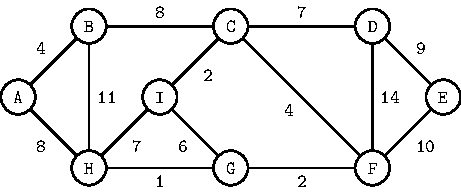
\includegraphics{mst}
\end{figure}

\paragraph{Analisi della complessità} \(\Omicron(m \log n)\)

L'efficienza dell'algoritmo di Prim dipende dalla coda con priorità.
Può essere implementato tramite heap binario oppure con un vettore non ordinato.

\subparagraph{heap binario}
Nel caso si utilizzi un heap binario allora:

\begin{itemize}[topsep=0pt, itemsep=0pt]
	\item[\circled{\ref{prim:init}}]
	l'inizializzazione costa \(\Omicron(m \log n)\);

	\item[\circled{\ref{prim:ciclo-esterno}}]
	il ciclo principale viene eseguito \(n-1\) per una complessità di \(\Omicron(n)\) volte dove ogni operazione di {\heapDeleteMin} costa \(\Omicron(\log n)\);

	\item[\circled{\ref{prim:ciclo-interno}}]
	il ciclo interno viene eseguito \(\Omicron(m)\) volte dove ogni operazione di {\heapDecrease} costa \(\Omicron(\log n)\).
\end{itemize}
Per un totale di \(\Omicron(n + m \log n + n \log n) = \Omicron(m \log n)\).

\begin{note}
L'algoritmo risulta asintoticamente uguale a quello di Kruskal.
\end{note}

\subparagraph{vettore non ordinato}
Nel caso si utilizzi vettore un non ordinato:
\begin{itemize}[topsep=0pt, itemsep=0pt]
	\item[\circled{\ref{prim:init}}]
	l'inizializzazione costa \(\Omicron(n)\);

	\item[\circled{\ref{prim:ciclo-esterno}}]
	il ciclo principale viene eseguito \(n-1\) per una complessità di \(\Omicron(n)\) volte dove ogni operazione di {\heapDeleteMin} costa \(\Omicron(n)\);

	\item[\circled{\ref{prim:ciclo-interno}}]
	il ciclo interno viene eseguito \(\Omicron(m)\) volte dove ogni operazione di {\heapDecrease} costa \(\Omicron(1)\).
\end{itemize}
Per un totale di \(\Omicron(n + n^2 + m \cdot 1) = \Omicron(n^2)\).

\begin{note}
Cambiando la struttura dati cambia la complessità dell'algoritmo.
\end{note}

In definitiva se il grafo è \emph{sparso} conviene utilizzare l'heap binario (\(\Omicron(m \log n)\)), mentre se il grafo è \emph{denso} (o addirittura completo) conviene utilizzare il vettore non ordinato (\(\Omicron(n^2)\)).

\subsection{Cenni storici}

\begin{figure}[H]
	\centering\footnotesize
	\begin{chronology}*[1]{1925}{1930}{.25\linewidth}
		\event{1926}{Boruvka}
		\event{1930}{Jarnik}
	\end{chronology}
	\begin{chronology}*[1]{1955}{1958}{.2\linewidth}
		\event{1956}{\color{purple}Kruskal}
		\event{1957}{\color{purple}Prim}
	\end{chronology}
	\begin{chronology}*[1]{1985}{1988}{.2\linewidth}
		\event{1987}{Fredman-Tarjan}
	\end{chronology}
	\begin{chronology}*[1]{1993}{1996}{.2\linewidth}
		\event{1995}{Karger, Klein, Tarjan}
	\end{chronology}
\end{figure}

L'algoritmo di Fredman-Tarjan sfrutta un heap di Fibonacci che abbassa di molto la complessità dell'algoritmo ma ha dei costi associati molto grandi e quindi non viene utilizzato.

Nel '95 Karger, Klein e Tarjan hanno ideato un algoritmo probabilistico che risolve il problema in \(\Omicron(m + n)\) (molto spesso andare \enquote{a caso} conviene).

Se questo problema si possa risolvere in tempo lineare in modo deterministico è una questione ancora aperta.

\subsection{Conclusioni}
Gli algoritmi ingordi sono semplici da programmare e molto efficienti.
Inoltre quando è possibile dimostrare la proprietà di scelta ingorda, danno la soluzione ottima.
Una soluzione sub-ottima è comunque accettabile.

\ifsubfile
\end{document}
\fi
